Essa disposição é vantajosa, pois sendo o indutor o órgão rotativo, pode ser alimentado com tensão baixa, o que facilita sua isolação.

\begin{figure}[ht!]
\center 
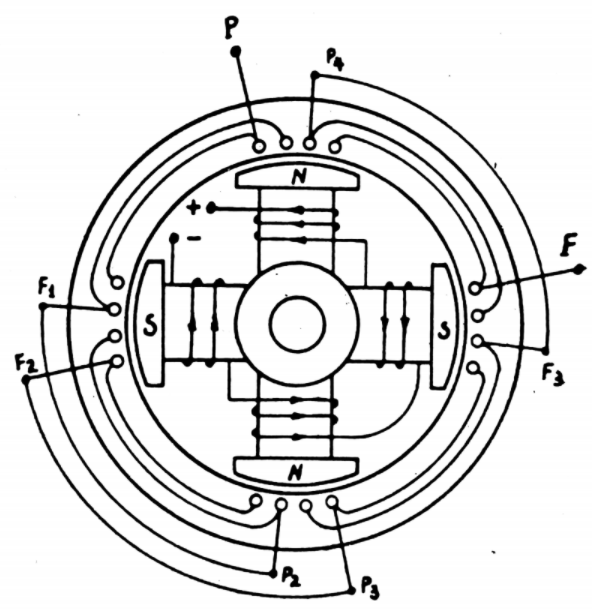
\includegraphics[scale=0.3]{imagens/7.PNG}
\caption{Alternador monofásico com 4 polos.}
\end{figure}

O indutor rotativo é constituído por uma roda, sobre a qual estão presos os núcleos polares com as bobinas de excitação. Estas bobinas são geralmente agrupadas em série, constituindo o circuito de excitação, cujos terminais são conectados a dois anéis coletores, os quais são eletricamente isolados, mas mecanicamente presos ao eixo do rotor. A alimentação do circuito de excitação é feita por meio de suas escovas apoiadas sobre os mencionados anéis coletores.

A energia destinada à alimentação do circuito de excitação pode ser fornecida por acumuladores ou por um dínamo acionado pelo próprio eixo do alternador.

Um elemento importante na determinação do número dos polos de um alternador é o número de rotações por minuto do motor de acionamento. Em geral os alternadores são acionados por motores à Diesel, turbinas hidráulicas e turbinas à vapor. Os motores à Diesel e as turbinas hidráulicas têm seu regime de funcionamento normal com velocidades que variam entre 200 e 700 rotações por minuto. Os alternadores de 60 $Hz$, acionados por esses motores e essas turbinas, devem possuir um número de polos que varia entre 10 e 36, pois:

Para uma velocidade de 200 RPM temos
$$\frac{2*60*60}{200} = 36 \text{ polos}$$

Para 700 RPM
$$\frac{2*60*60}{700} = 10 \text{ polos}$$

